\chapter{Projektowanie bazy danych}
\section{Baza danych}

Bazy danych stanowią kluczowy element wielu aplikacji. Pozwalają one na przechowywanie, organizowanie i zarządzanie danymi. Można łatwo do bazy danych dodawać nowe dane i rekordy co sprawia że aplikację można dalej rozwijać. Bazy danych wykorzystują struktury które są zoptymalizowane pod kątem przeszukiwania i pobierania danych. Dodatkowo istnieje wiele narzędzi które pozwalają na integracje z bazami danych takich jak SpringBoot i Hibernate % TU chyba powinna być referencja do rozdziału/tabeli *tabela roz3*)

Do zaprojektowania bazy danych został wykonany diagram związków encji który pokazuję jakiego typu dane są użyte w jakich tabelach oraz jakie są relacje miedzy tymi tabelami.
% TO DO: ciekaw jestem, jak zapewniona zostanie unikalność kluczy w device_core (bo tam pojawią się identyfikatory z trzech innych tabel, a więc musi być jakiś mechanizm, by te identyfikatory się nie powtórzyły w tych tabelach).
\begin{figure}[h]
    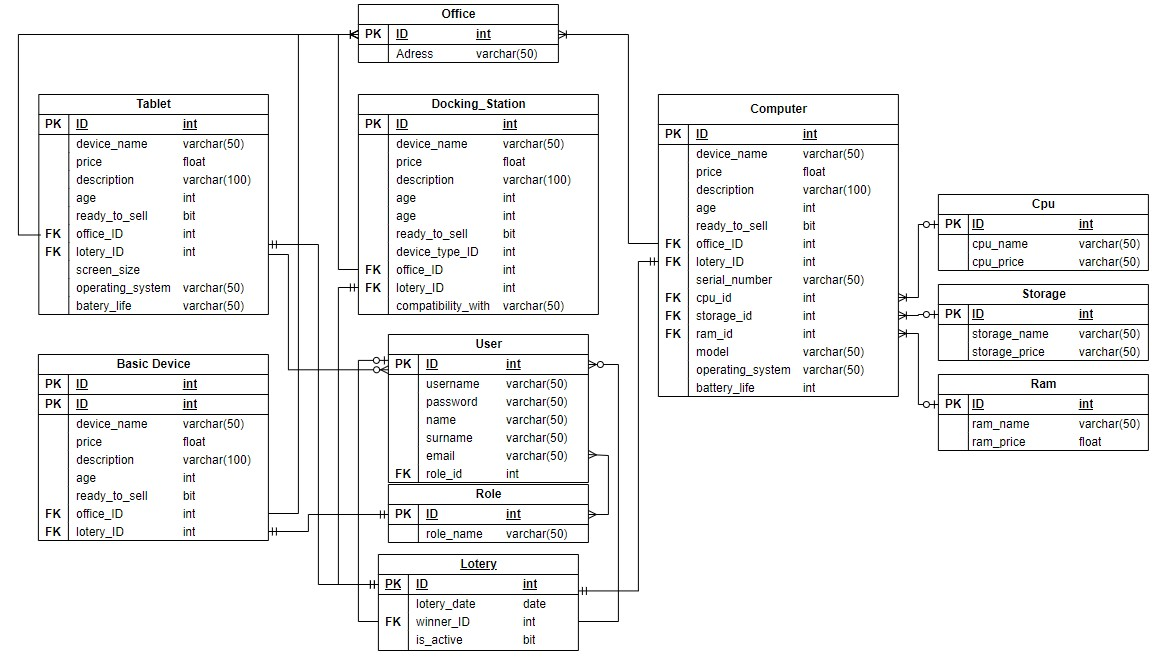
\includegraphics[width=\linewidth]{rys04/ER_Diagram.jpg} % TO DO: prosiłem o wektory, a nie bitmapy (a jeśli bitmapy, to nie jpg!!!)
    \caption{Diagram związków encji}
    \label{ErDiagram_etykieta}
\end{figure}


W bazie danych istnieją 4 rodzaje urządzeń:
\begin{itemize}
	\item Podstawowe urządzenie
	\item Komputer
	\item Tablet
	\item Stacja dokująca
\end{itemize}
Podstawowe urządzenie pozwala na dodanie do bazy danych urządzenia nie wliczającego się do pozostałych typów.
Wszystkie te 4 typy urządzeń mają taką samą funkcje w systemie czyli losowanie i odsprzedaż urządzenia. Każda z tabel: Basic Device, Computer, Tablet, Docking\_Station zawiera podobne pola które system potrzebuje do stworzenia losowania oraz opisania stanu technicznego urządzeń. Polami wspólnymi dla 4 typów urządzeń są:
\begin{itemize}
	\item Nazwa urządzenia
	\item Cena urządzenia
	\item Opis, czyli stan techniczny i dodatkowe uwagi
	\item Wiek urządzenia
	\item Informacja czy sprzęt jest gotowy do odsprzedaży, czy przeszedł inwentaryzacje
	\item Biuro w którym znajduje się urządzenie
	\item Opcjonalnie loteria w której będzie losowane to urządzenie
\end{itemize}

Istnieją też pola które pozwalają na dokładniejszy opis urządzenia ze względu na jego typ. Stacja dokująca posiada informacje do jakiego typu komputera można ją podłączyć. Tablet za to rozmiar ekranu, system operacyjny i żywotność baterii.
 Komputer posiada największą liczbę informacji, jest on sprzętem najczęściej sprzedawanym w firmach dlatego też otrzymał największe wsparcie w systemie. Oprócz informacji takich jak numer seryjny, system, żywotność baterii czy model komputer w bazie danych połączony jest z tabelami dotyczącymi Procesora, pamięci, czy pamięci RAM. Takie połączenie pozwala na podpowiadanie nazwy komponentu komputera biorąc informacje o komponentach z bazy danych. Komponenty te reprezentowane przez tabele Cpu, Storage i Ram posiadają tylko informacje o nazwie i cenie. Cena komponentów pomaga oszacować ostateczną cenę komputera.
Tabelą wykorzystywaną do losowania, archiwizowania i ustalania daty losowania jest tabela Lotery. Przechowuje ona informacje o dacie, o tym czy losowanie jest aktywne oraz zwycięzce losowania.
W systemie istnieją dwie role Administrator i Pracownik. Wykorzystanie tabeli Role pozwala na dodaniu dodatkowych ról w systemie w przyszłym rozwoju aplikacji. Użytkownik posiada swoje dane jak nazwa użytkownika, imię nazwisko oraz email firmowy. Email firmowy jest niezbędny do założenia konta, brania udziału w loterii.